% ==============================================================================
% TCC - Nome do Aluno
% Capítulo 1 - Introdução
% ==============================================================================
\chapter{Introdução}
\label{sec-intro}
Na computação muitas aplicações necessitam considerar um conjunto de conexões entre dados e uso de algoritmos sobre esses dados para poder responder perguntas, como exemplo, se existe um caminho entre dois dados distintos seguindo por essas conexões, qual a menor distância entre eles ou ainda quantos dados podemos alcançar a partir de um outro determinado dado. Para modelar tais situações, utilizamos um tipo abstrato chamado grafo \cite{ziviani2004projeto}. Um grafo G = (V,E) consiste de um conjunto não vazio V de vértices, que representam os dados, e um conjunto que pode ser vazio de arestas E, que representam a ligação entre esses dados. A figura \ref{fig-intro-exemplografo} mostra um exemplo de um grafo. Exemplos de modelagens por grafos são a ligação entre cidades em que as arestas representam as distâncias entre elas e a representação de uma rede interna de computadores. 

\begin{figure}[H]
\centering
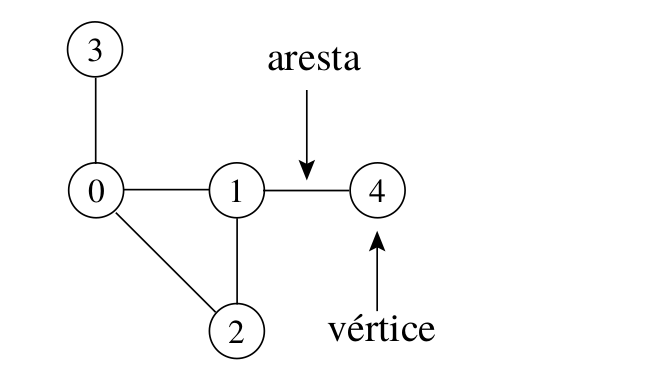
\includegraphics[width=.65\textwidth]{figuras/grafo-exemplo} 
\caption{Exemplo de um grafo.}
\label{fig-intro-exemplografo}
\end{figure}

Um problema clássico da literatura envolvendo grafos é o cálculo de caminho mínimo \cite{moura2010estudo}. Nele desejamos obter o menor caminho entre dois pontos específicos do grafo representado. A sua modelagem é feita representando as arestas com determinados pesos que podem significar o tempo decorrente entre executar tarefas, o custo de transmitir informações entre locais, quantidades específicas a serem transportadas entre um local e outro e etc \cite{drozdek2012data}. 

Dentre as modelagens realizadas para resolver o problema do caminho mínimo, uma muito utilizada é a definição do menor caminho entre dois pontos geográficos tendo como aplicação prática o uso de softwares do tipo GPS. Nela representamos as interseções das ruas, caminhos ou rodovias como o vértices do grafo e as distâncias entre essas interseções (as próprias ruas, caminhos ou rodovias) como as arestas e tendo seus respectivos pesos como sendo a distâncias entre essas interseções.

%A figura X mostra o exemplo desta modelagem abordada [a ser colocado ainda professora].

A motivação deste trabalho é o estudo dos algoritmos de menor caminho em grafos, desde os clássicos como o algoritmo de Dijkstra \cite{dijkstra1959note} até algoritmos mais recentes propostos como o \textit{Anytime Dynamic} A* (AD*) \cite{likhachev2008anytime}. Tem por  objetivo verificar o desempenho e a eficácia destes algoritmos, averiguar o impacto que as estruturas de dados utilizadas para resolver o problema causam e analisar quais situações os algoritmos estudados melhor se aplicam.

\section{Revisão bibliográfica e trabalhos correlatos}
\label{sec-intro-correlatos}
O algoritmo de Dijkstra é amplamente difundido na literatura, sendo que é utilizado como base para o estudo desse algoritmo os livros de \citeonline{cormen2009introduction} e \citeonline{drozdek2012data}, em que abordam a descrição do algoritmo, estruturas de dados e a análise computacional das mesmas.

O algoritmo A* é bastante difundido na literatura. Foi proposto por \citeonline{hart1968formal}. Ele é descrito no livro de \citeonline{russell1995modern} e no artigo de \citeonline{likhachev2008anytime}. O pseudo-código descrito neste livro e artigo são usados como base para a implementação desse algoritmo neste projeto.

O estudo dos algoritmos ARA* e AD* é baseado no artigo no qual esses algoritmos foram propostos \cite{likhachev2008anytime}, além do artigo em que investiga esses algoritmos \cite{moura2010estudo}.

O trabalho de \citeonline{larkin2014back} analisa o uso de diversas estruturas de dados como fila de prioridades e seus respectivos impactos, ressaltando diferenças entre a proposta teórica dessas estruturas e a aplicação prática.
\section{Metodologia de pesquisa}
\label{sec-intro-metodologia}
Todos os algoritmos estudados foram implementados na linguagem Java, a versão do compilador utilizado é Java 1.8.0\_131. Os testes a serem realizados e as instâncias utilizadas estão descritos no capítulo \ref{sec-testes}.
\newpage
\section{Organização dos capítulos}
\label{sec-intro-organizaocao}
Nos próximos capítulos este trabalho está estruturado da seguinte forma:
\begin{description}
%\item[Capítulo \ref{sec-intro}:] Esta introdução.
\item[Capítulo \ref{sec-algoritmosestaticos}:] Apresenta a descrição do algoritmo clássico de Dijkstra, as versões implementadas baseadas em estrutura de dados diferentes e suas respectivas descrições. Apresenta também a descrição do algoritmo busca A*, sua diferença em relação ao Dijkstra e uma descrição do uso da estratégia de heurísticas e como elas são classificadas;
\item[Capítulo \ref{sec-dinamicos}:] Apresenta a descrição dos algoritmos ARA* e AD*, a estratégia de heurística inflada e uma breve descrição de grafos dinâmicos, nos quais o algoritmo AD* se aplica;
\item[Capítulo \ref{sec-testes}:] Apresenta a descrição dos testes realizados, seus respectivos resultados e uma análise desses para cada algoritmo abordado;
\item[Capítulo \ref{sec-conclusao}:] Traz a conclusão geral deste trabalho e possíveis trabalhos futuros.
\end{description}